\documentclass[dvipdfmx]{article}
\usepackage{mathpazo}
\usepackage{amsmath,amssymb}
\usepackage{array}
\usepackage[hiresbb]{graphicx}
\usepackage{textcomp}
\usepackage{dcolumn}
\usepackage{here}
\usepackage{lscape}
\usepackage[top=30truemm,bottom=30truemm,left=25truemm,right=25truemm]{geometry}
\begin{document}

\title{Results}
\author{Reio.T}
\date{9/27/2018}
\maketitle

\normalsize
\setlength\intextsep{0pt}

Data = from 1957 to 2017 ($n=53090$)

\section{Full-sample analysis}


\begin{itemize}
  \item Batting-Average
  ($n=17788$)
   \begin{center}

    \begin{figure}[H]
     \centering
     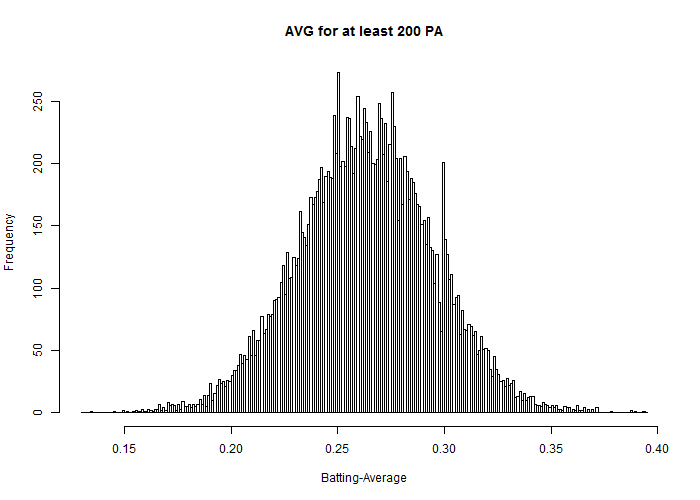
\includegraphics[width = 14cm, height = 10cm]{graphs/AVG_200PA.png}
    \end{figure}


     *difference between the number of batters with .299 (0.37\%)
     and .300 (1.13\%) is significant at 0.1\% ($\chi^2 = 69.03$)

     **Also, the difference between those with .299, .298 (0.87\%)
     and with .300 and .301 (1.91\%) is significant at 0.1\%
     ($\chi^2 = 70.26$)

   \end{center}

  \item Other Index for performance

  \begin{figure}[H]
   \centering
   \begin{tabular}{cc}
    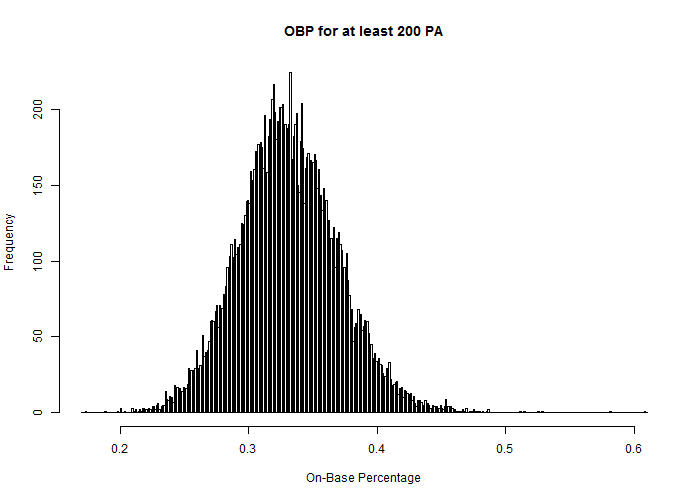
\includegraphics[width = 8cm, height = 6cm]{graphs/OBP_200PA.png} &
    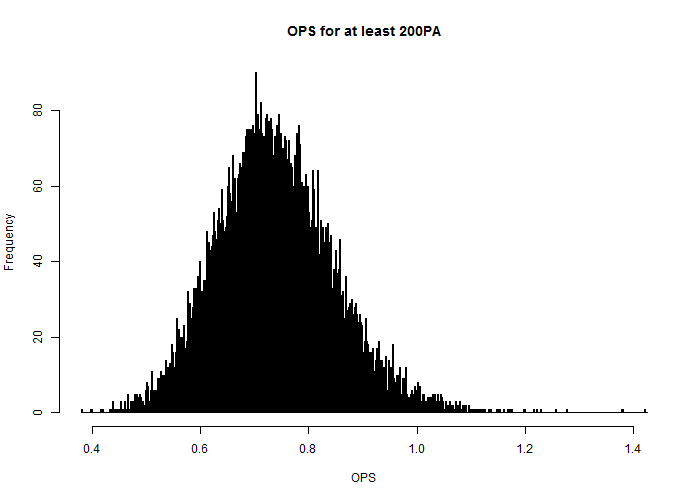
\includegraphics[width = 8cm, height = 6cm]{graphs/OPS_200PA.png} \\
    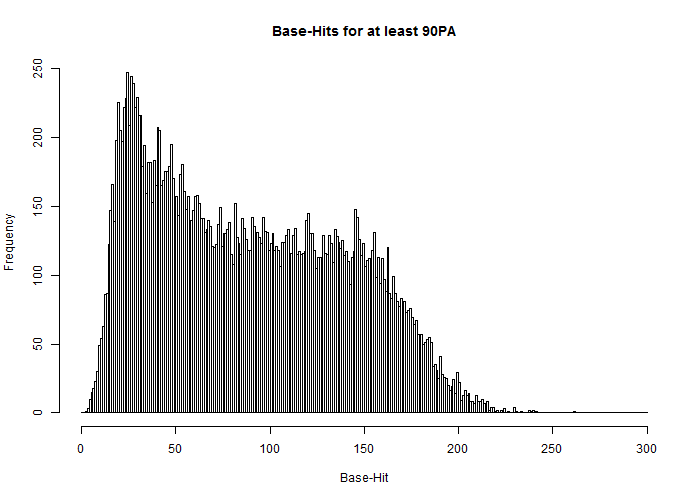
\includegraphics[width = 8cm, height = 6cm]{graphs/H_90PA.png} &
    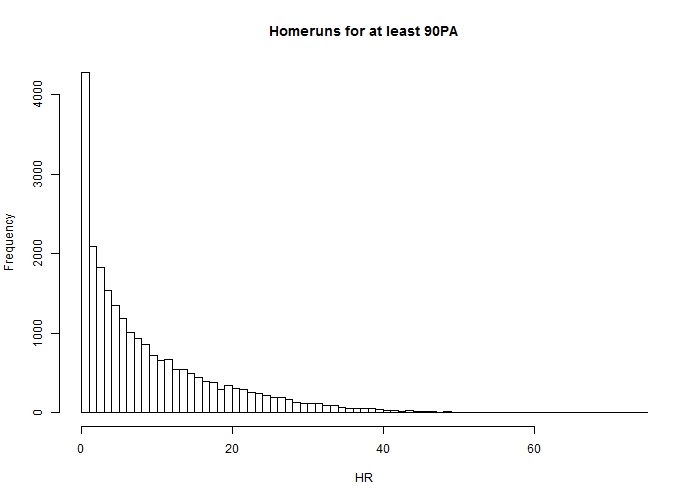
\includegraphics[width = 8cm, height = 6cm]{graphs/HR_90PA.png} \\
    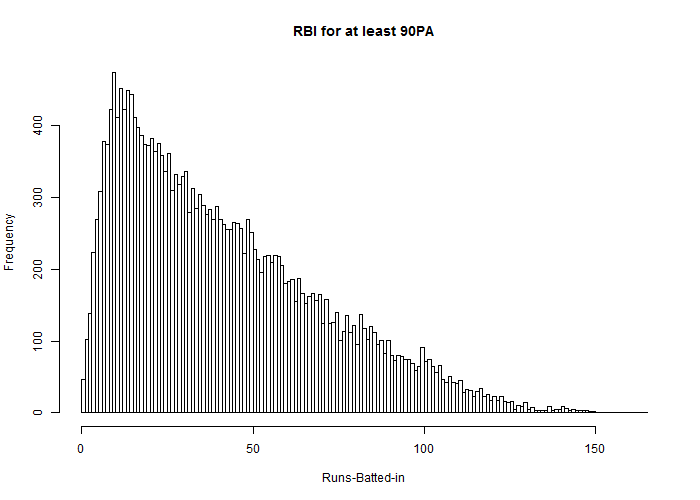
\includegraphics[width = 8cm, height = 6cm]{graphs/RBI_90PA.png} &
    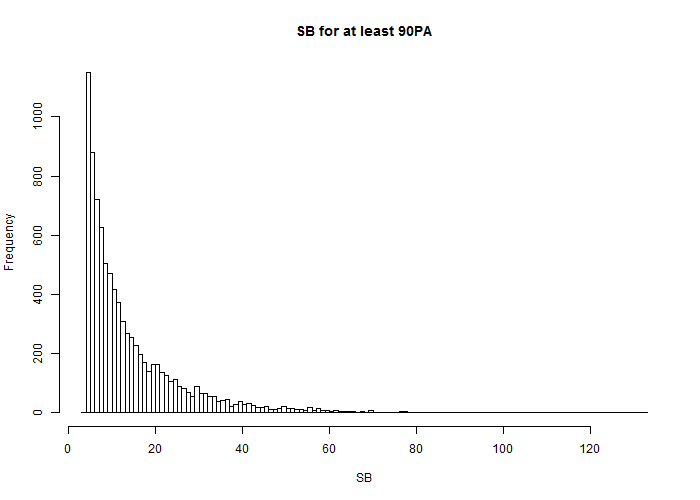
\includegraphics[width = 8cm, height = 6cm]{graphs/SB_5SB.png} \\
   \end{tabular}
 \end{figure}



  \begin{landscape}
   
% Table created by stargazer v.5.2.2 by Marek Hlavac, Harvard University. E-mail: hlavac at fas.harvard.edu
% Date and time: ��, 9 25, 2018 - 13:12:50
\begin{table}[!htbp] \centering
  \caption{}
  \label{}
  \scriptsize
\begin{tabular}{@{\extracolsep{5pt}}lcccccc}
\\[-1.8ex]\hline
\hline \\[-1.8ex]
 & \multicolumn{6}{c}{\textit{Dependent variable:}} \\
\cline{2-7}
\\[-1.8ex] & \multicolumn{6}{c}{L\_Sal} \\
\\[-1.8ex] & (1) & (2) & (3) & (4) & (5) & (6)\\
\hline \\[-1.8ex]
 AVG\_87 & 9.849$^{***}$ &  &  &  &  &  \\
  & (0.616) &  &  &  &  &  \\
  & & & & & & \\
 OBP\_87 &  & 10.439$^{***}$ &  &  &  &  \\
  &  & (0.453) &  &  &  &  \\
  & & & & & & \\
 OPS\_87 &  &  & 4.999$^{***}$ &  &  &  \\
  &  &  & (0.162) &  &  &  \\
  & & & & & & \\
 wOBA &  &  &  & 11.610$^{***}$ &  &  \\
  &  &  &  & (0.423) &  &  \\
  & & & & & & \\
 BATTING &  &  &  &  & 0.031$^{***}$ &  \\
  &  &  &  &  & (0.001) &  \\
  & & & & & & \\
 fWAR &  &  &  &  &  & 0.272$^{***}$ \\
  &  &  &  &  &  & (0.009) \\
  & & & & & & \\
 ABOVE\_300 & $-$0.842 & $-$0.481 & $-$0.207 & $-$0.565 & $-$0.070 & 0.043 \\
  & (0.767) & (0.438) & (0.336) & (0.409) & (0.055) & (0.071) \\
  & & & & & & \\
 FIELDING & 0.003$^{*}$ & 0.005$^{***}$ & 0.007$^{***}$ & 0.006$^{***}$ & 0.007$^{***}$ &  \\
  & (0.002) & (0.002) & (0.002) & (0.002) & (0.002) &  \\
  & & & & & & \\
 BaseRun & $-$0.021$^{***}$ & $-$0.022$^{***}$ & $-$0.014$^{***}$ & $-$0.017$^{***}$ & $-$0.017$^{***}$ &  \\
  & (0.005) & (0.005) & (0.005) & (0.005) & (0.005) &  \\
  & & & & & & \\
 AVG\_87:ABOVE\_300 & 3.058 &  &  &  &  &  \\
  & (2.456) &  &  &  &  &  \\
  & & & & & & \\
 OBP\_87:ABOVE\_300 &  & 1.515 &  &  &  &  \\
  &  & (1.164) &  &  &  &  \\
  & & & & & & \\
 OPS\_87:ABOVE\_300 &  &  & 0.165 &  &  &  \\
  &  &  & (0.389) &  &  &  \\
  & & & & & & \\
 wOBA:ABOVE\_300 &  &  &  & 1.483 &  &  \\
  &  &  &  & (1.092) &  &  \\
  & & & & & & \\
 BATTING:ABOVE\_300 &  &  &  &  & 0.001 &  \\
  &  &  &  &  & (0.002) &  \\
  & & & & & & \\
 fWAR:ABOVE\_300 &  &  &  &  &  & $-$0.012 \\
  &  &  &  &  &  & (0.018) \\
  & & & & & & \\
 Constant & 11.618$^{***}$ & 10.750$^{***}$ & 10.485$^{***}$ & 10.417$^{***}$ & 14.187$^{***}$ & 13.778$^{***}$ \\
  & (0.160) & (0.149) & (0.121) & (0.137) & (0.014) & (0.019) \\
  & & & & & & \\
\hline \\[-1.8ex]
Observations & 8,883 & 8,883 & 8,883 & 8,883 & 8,883 & 8,928 \\
R$^{2}$ & 0.065 & 0.101 & 0.146 & 0.125 & 0.140 & 0.153 \\
Adjusted R$^{2}$ & 0.064 & 0.100 & 0.146 & 0.125 & 0.140 & 0.153 \\
Residual Std. Error & 1.295 (df = 8877) & 1.270 (df = 8877) & 1.238 (df = 8877) & 1.253 (df = 8877) & 1.242 (df = 8877) & 1.231 (df = 8924) \\
F Statistic & 122.451$^{***}$ (df = 5; 8877) & 199.008$^{***}$ (df = 5; 8877) & 304.053$^{***}$ (df = 5; 8877) & 254.613$^{***}$ (df = 5; 8877) & 290.119$^{***}$ (df = 5; 8877) & 539.388$^{***}$ (df = 3; 8924) \\
\hline
\hline \\[-1.8ex]
\textit{Note:}  & \multicolumn{6}{r}{$^{*}$p$<$0.1; $^{**}$p$<$0.05; $^{***}$p$<$0.01} \\
\end{tabular}
\end{table}

  \end{landscape}


   \begin{landscape}
     
% Table created by stargazer v.5.2.2 by Marek Hlavac, Harvard University. E-mail: hlavac at fas.harvard.edu
% Date and time: ��, 9 28, 2018 - 10:08:16
\begin{table}[!htbp] \centering
  \caption{}
  \label{}
  \scriptsize
\begin{tabular}{@{\extracolsep{5pt}}lcccccc}
\\[-1.8ex]\hline
\hline \\[-1.8ex]
 & \multicolumn{6}{c}{\textit{Dependent variable:}} \\
\cline{2-7}
\\[-1.8ex] & \multicolumn{6}{c}{Log-salary next season} \\
\\[-1.8ex] & \multicolumn{2}{c}{\textit{OLS}} & \multicolumn{4}{c}{\textit{felm}} \\
\\[-1.8ex] & (1) & (2) & (3) & (4) & (5) & (6)\\
\hline \\[-1.8ex]
 fWAR & 0.272$^{***}$ & 0.281$^{***}$ & 0.279$^{***}$ & 0.102$^{***}$ & 0.022$^{*}$ & 0.083$^{***}$ \\
  & (0.009) & (0.008) & (0.008) & (0.010) & (0.012) & (0.008) \\
  & & & & & & \\
 ABOVE\_300 & 0.043 & $-$0.089 & $-$0.102$^{*}$ & $-$0.038 & $-$0.156$^{**}$ & $-$0.077$^{*}$ \\
  & (0.071) & (0.062) & (0.062) & (0.072) & (0.070) & (0.045) \\
  & & & & & & \\
 AGE &  & 0.928$^{***}$ & 0.932$^{***}$ &  &  & 1.619$^{***}$ \\
  &  & (0.034) & (0.034) &  &  & (0.027) \\
  & & & & & & \\
 AGE\_sq &  & $-$0.013$^{***}$ & $-$0.013$^{***}$ &  &  & $-$0.024$^{***}$ \\
  &  & (0.001) & (0.001) &  &  & (0.0005) \\
  & & & & & & \\
 WPA &  &  &  &  & 15.549$^{***}$ & 7.584$^{***}$ \\
  &  &  &  &  & (1.530) & (0.988) \\
  & & & & & & \\
 nWPA &  &  &  &  & 24.902$^{***}$ & 20.865$^{***}$ \\
  &  &  &  &  & (1.571) & (1.018) \\
  & & & & & & \\
 fWAR:ABOVE\_300 & $-$0.012 & 0.004 & 0.006 & 0.0003 & 0.031$^{*}$ & 0.001 \\
  & (0.018) & (0.015) & (0.015) & (0.017) & (0.017) & (0.011) \\
  & & & & & & \\
 Constant & 13.778$^{***}$ & $-$1.664$^{***}$ &  &  &  &  \\
  & (0.019) & (0.498) &  &  &  &  \\
  & & & & & & \\
\hline \\[-1.8ex]
Fixed effect & - & - & Team & Individual & Individual, Team & Team \\
Observations & 8,928 & 8,928 & 8,928 & 8,928 & 8,928 & 8,928 \\
R$^{2}$ & 0.153 & 0.358 & 0.366 & 0.484 & 0.521 & 0.802 \\
Adjusted R$^{2}$ & 0.153 & 0.357 & 0.363 & 0.364 & 0.407 & 0.755 \\
Residual Std. Error & 1.231 (df = 8924) & 1.073 (df = 8922) & 1.068 (df = 8893) & 1.067 (df = 7239) & 1.030 (df = 7208) & 0.663 (df = 7206) \\
F Statistic & 539.388$^{***}$ (df = 3; 8924) & 993.022$^{***}$ (df = 5; 8922) &  &  &  &  \\
\hline
\hline \\[-1.8ex]
\textit{Note:}  & \multicolumn{6}{r}{$^{*}$p$<$0.1; $^{**}$p$<$0.05; $^{***}$p$<$0.01} \\
\end{tabular}
\end{table}


     
% Table created by stargazer v.5.2.2 by Marek Hlavac, Harvard University. E-mail: hlavac at fas.harvard.edu
% Date and time: ��, 9 28, 2018 - 10:08:21
\begin{table}[!htbp] \centering
  \caption{}
  \label{}
  \scriptsize
\begin{tabular}{@{\extracolsep{5pt}}lcccccc}
\\[-1.8ex]\hline
\hline \\[-1.8ex]
 & \multicolumn{6}{c}{\textit{Dependent variable:}} \\
\cline{2-7}
\\[-1.8ex] & \multicolumn{6}{c}{Log-salary next season} \\
\\[-1.8ex] & \multicolumn{2}{c}{\textit{OLS}} & \multicolumn{4}{c}{\textit{felm}} \\
\\[-1.8ex] & (1) & (2) & (3) & (4) & (5) & (6)\\
\hline \\[-1.8ex]
 BATTING & 0.031$^{***}$ & 0.030$^{***}$ & 0.030$^{***}$ & 0.030$^{***}$ & 0.013$^{***}$ & 0.015$^{***}$ \\
  & (0.001) & (0.001) & (0.001) & (0.001) & (0.002) & (0.001) \\
  & & & & & & \\
 ABOVE\_300 & $-$0.070 & $-$0.112$^{**}$ & $-$0.099$^{**}$ & $-$0.108$^{**}$ & $-$0.187$^{***}$ & $-$0.177$^{***}$ \\
  & (0.055) & (0.049) & (0.049) & (0.049) & (0.054) & (0.044) \\
  & & & & & & \\
 FIELDING & 0.007$^{***}$ & 0.008$^{***}$ & 0.008$^{***}$ & 0.008$^{***}$ & $-$0.004$^{**}$ & 0.007$^{***}$ \\
  & (0.002) & (0.002) & (0.002) & (0.002) & (0.002) & (0.001) \\
  & & & & & & \\
 BaseRun & $-$0.017$^{***}$ & 0.007$^{*}$ & 0.001 & 0.002 & $-$0.048$^{***}$ & $-$0.003 \\
  & (0.005) & (0.004) & (0.005) & (0.005) & (0.006) & (0.004) \\
  & & & & & & \\
 AGE &  & 0.947$^{***}$ & 0.971$^{***}$ & 0.976$^{***}$ &  & 1.008$^{***}$ \\
  &  & (0.035) & (0.035) & (0.035) &  & (0.032) \\
  & & & & & & \\
 AGE\_sq &  & $-$0.014$^{***}$ & $-$0.014$^{***}$ & $-$0.014$^{***}$ &  & $-$0.015$^{***}$ \\
  &  & (0.001) & (0.001) & (0.001) &  & (0.001) \\
  & & & & & & \\
 WPA &  &  &  &  & 10.820$^{***}$ & 16.259$^{***}$ \\
  &  &  &  &  & (1.629) & (1.373) \\
  & & & & & & \\
 nWPA &  &  &  &  & 25.727$^{***}$ & 44.336$^{***}$ \\
  &  &  &  &  & (1.492) & (0.982) \\
  & & & & & & \\
 BATTING:ABOVE\_300 & 0.001 & 0.002 & 0.002 & 0.001 & 0.003 & 0.006$^{***}$ \\
  & (0.002) & (0.002) & (0.002) & (0.002) & (0.002) & (0.002) \\
  & & & & & & \\
 Constant & 14.187$^{***}$ & $-$1.393$^{***}$ &  &  &  &  \\
  & (0.014) & (0.519) &  &  &  &  \\
  & & & & & & \\
\hline \\[-1.8ex]
Fixed effect & - & - & Position & Position, Team & Individual,Position, Team & Position, Team \\
Observations & 8,883 & 8,883 & 8,883 & 8,883 & 8,883 & 8,883 \\
R$^{2}$ & 0.140 & 0.324 & 0.344 & 0.354 & 0.548 & 0.476 \\
Adjusted R$^{2}$ & 0.140 & 0.324 & 0.343 & 0.350 & 0.439 & 0.473 \\
Residual Std. Error & 1.242 (df = 8877) & 1.101 (df = 8875) & 1.086 (df = 8863) & 1.080 (df = 8834) & 1.003 (df = 7151) & 0.972 (df = 8832) \\
F Statistic & 290.119$^{***}$ (df = 5; 8877) & 608.849$^{***}$ (df = 7; 8875) &  &  &  &  \\
\hline
\hline \\[-1.8ex]
\textit{Note:}  & \multicolumn{6}{r}{$^{*}$p$<$0.1; $^{**}$p$<$0.05; $^{***}$p$<$0.01} \\
\end{tabular}
\end{table}

   \end{landscape}

  \end{itemize}

 \section{Restricted-sample andalysis}

 Behavior of the players may be influenced by the Season-specific effect.

 Now I devide sample year into 4 era, according to three important
 events for the players' contract:

  \begin{itemize}
    \item Before ``Free Agent'' system was introduced: -1975
    ($n = 4292$)

    \item Before ``Strike'' of the players occurred: 1976-1994
    ($n = 5331$)

    \item Before `\textit{Moneyball}` was published: 1995-2001
    ($n = 2028$)

    \item After `\textit{Moneyball}`: 2002-
    ($n = 5555$)
  \end{itemize}

 \begin{figure}[H]
   \centering

   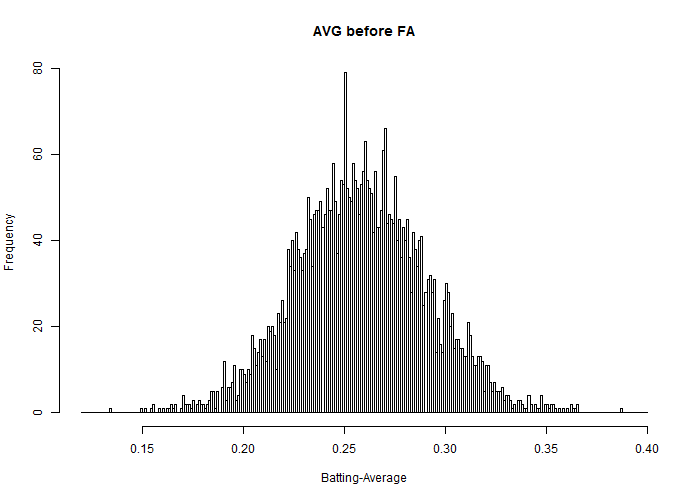
\includegraphics[width = 14cm, height = 10cm]{graphs/AVG_bffa.png}

   .299 to .300: significant at 5\% ($\chi^2 = 3.04, p = 0.0406$)

   .298, .299 to .300, .301: significant at 1\% ($\chi^2 = 7.34, p = 0.0034$)
 \end{figure}

 \begin{figure}[H]
   \centering
   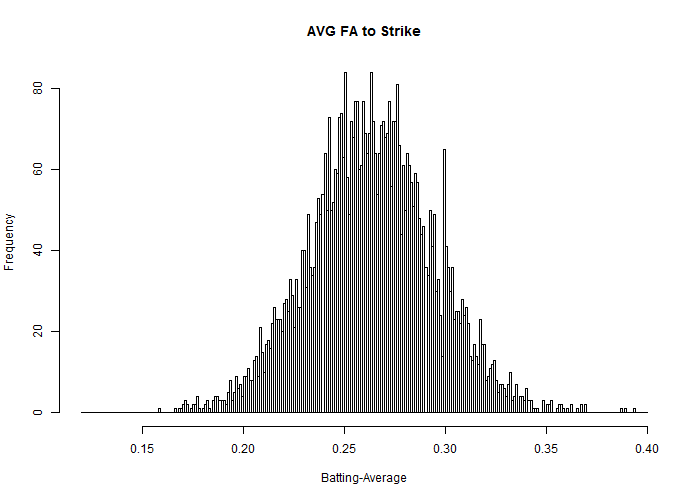
\includegraphics[width = 14cm, height = 10cm]
   {graphs/AVG_fast}

   .299 to .300: significant at 0.1\% ($\chi^2 = 31.88$)

   .298, .299 to .300, .301: significant at 0.1\% ($\chi^2 = 31.60$)

 \end{figure}

 \begin{figure}[H]
   \centering
   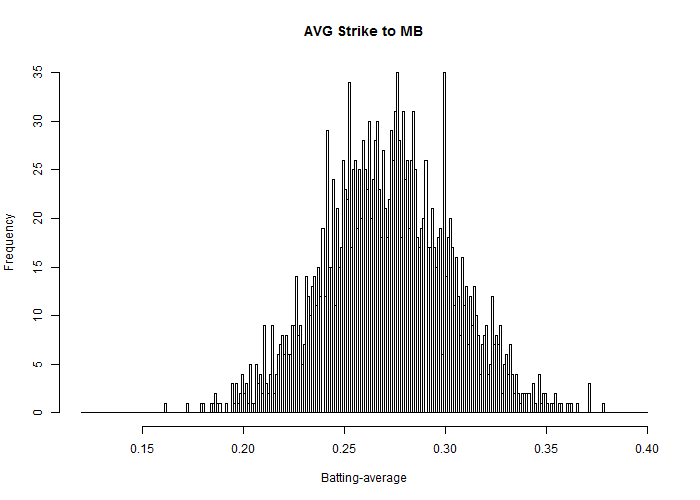
\includegraphics[width = 14cm, height = 10cm]
   {graphs/AVG_stmb}

   .299 to .300: significant at 0.1\% ($\chi^2 = 19.32$)

   .298, .299 to .300, .301: significant at 1\% ($\chi^2 = 7.28, p = 0.0034$)
 \end{figure}

 \begin{figure}[H]
   \centering
   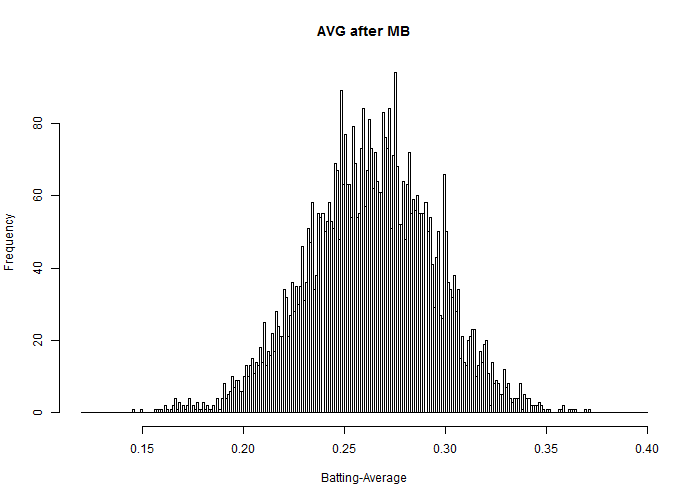
\includegraphics[width = 14cm, height = 10cm]
   {graphs/AVG_afmb}

   .299 to .300: significant at 0.1\% ($\chi^2 = 16.67$)

   .298, .299 to .300, .301: significant at 0.1\% ($\chi^2 = 23.10$)
 \end{figure}

 \begin{landscape}
   
% Table created by stargazer v.5.2.2 by Marek Hlavac, Harvard University. E-mail: hlavac at fas.harvard.edu
% Date and time: ��, 9 25, 2018 - 11:04:42
\begin{table}[!htbp] \centering
  \caption{}
  \label{}
  \scriptsize
\begin{tabular}{@{\extracolsep{5pt}}lcccccc}
\\[-1.8ex]\hline
\hline \\[-1.8ex]
 & \multicolumn{6}{c}{\textit{Dependent variable:}} \\
\cline{2-7}
\\[-1.8ex] & \multicolumn{6}{c}{Log-salary next season} \\
\\[-1.8ex] & \multicolumn{2}{c}{\textit{OLS}} & \multicolumn{4}{c}{\textit{felm}} \\
\\[-1.8ex] & (1) & (2) & (3) & (4) & (5) & (6)\\
\hline \\[-1.8ex]
 fWAR\_bfst & 0.234$^{***}$ & 0.234$^{***}$ & 0.236$^{***}$ & 0.124$^{***}$ & 0.122$^{***}$ & 0.062$^{***}$ \\
  & (0.014) & (0.012) & (0.012) & (0.010) & (0.010) & (0.013) \\
  & & & & & & \\
 ABOVE\_300\_bfst & 0.154 & 0.013 & $-$0.003 & 0.138$^{*}$ & 0.114 & 0.168$^{**}$ \\
  & (0.120) & (0.104) & (0.104) & (0.078) & (0.078) & (0.075) \\
  & & & & & & \\
 AGE\_bfst &  & 0.812$^{***}$ & 0.811$^{***}$ & 1.872$^{***}$ & 1.879$^{***}$ & 1.829$^{***}$ \\
  &  & (0.054) & (0.054) & (0.061) & (0.062) & (0.060) \\
  & & & & & & \\
 AGE\_sq\_bfst &  & $-$0.012$^{***}$ & $-$0.012$^{***}$ & $-$0.027$^{***}$ & $-$0.027$^{***}$ & $-$0.026$^{***}$ \\
  &  & (0.001) & (0.001) & (0.001) & (0.001) & (0.001) \\
  & & & & & & \\
 WPA\_bfst &  &  &  &  &  & 0.025$^{**}$ \\
  &  &  &  &  &  & (0.012) \\
  & & & & & & \\
 nWPA\_bfst &  &  &  &  &  & $-$0.080$^{***}$ \\
  &  &  &  &  &  & (0.007) \\
  & & & & & & \\
 fWAR\_bfst:ABOVE\_300\_bfst & $-$0.007 & 0.015 & 0.017 & $-$0.037$^{**}$ & $-$0.033$^{*}$ & $-$0.027 \\
  & (0.030) & (0.026) & (0.026) & (0.019) & (0.019) & (0.018) \\
  & & & & & & \\
 Constant & 13.047$^{***}$ & $-$0.294 &  &  &  &  \\
  & (0.030) & (0.790) &  &  &  &  \\
  & & & & & & \\
\hline \\[-1.8ex]
Fixed effect & None & None & Team & Individual & Team + Individual & Team + Individual \\
Observations & 2,122 & 2,122 & 2,122 & 2,122 & 2,122 & 2,122 \\
R$^{2}$ & 0.189 & 0.401 & 0.416 & 0.837 & 0.844 & 0.856 \\
Adjusted R$^{2}$ & 0.188 & 0.399 & 0.407 & 0.778 & 0.784 & 0.800 \\
Residual Std. Error & 0.959 (df = 2118) & 0.825 (df = 2116) & 0.820 (df = 2089) & 0.502 (df = 1556) & 0.495 (df = 1529) & 0.476 (df = 1527) \\
F Statistic & 165.009$^{***}$ (df = 3; 2118) & 282.841$^{***}$ (df = 5; 2116) &  &  &  &  \\
\hline
\hline \\[-1.8ex]
\textit{Note:}  & \multicolumn{6}{r}{$^{*}$p$<$0.1; $^{**}$p$<$0.05; $^{***}$p$<$0.01} \\
\end{tabular}
\end{table}


   
% Table created by stargazer v.5.2.2 by Marek Hlavac, Harvard University. E-mail: hlavac at fas.harvard.edu
% Date and time: ��, 9 25, 2018 - 11:04:47
\begin{table}[!htbp] \centering
  \caption{}
  \label{}
  \scriptsize 
\begin{tabular}{@{\extracolsep{5pt}}lcccccc}
\\[-1.8ex]\hline
\hline \\[-1.8ex]
 & \multicolumn{6}{c}{\textit{Dependent variable:}} \\
\cline{2-7}
\\[-1.8ex] & \multicolumn{6}{c}{Log-salary next season} \\
\\[-1.8ex] & \multicolumn{2}{c}{\textit{OLS}} & \multicolumn{4}{c}{\textit{felm}} \\
\\[-1.8ex] & (1) & (2) & (3) & (4) & (5) & (6)\\
\hline \\[-1.8ex]
 BATTING\_bfst & 0.027$^{***}$ & 0.026$^{***}$ & 0.027$^{***}$ & 0.028$^{***}$ & 0.015$^{***}$ & 0.011$^{***}$ \\
  & (0.002) & (0.002) & (0.002) & (0.002) & (0.002) & (0.002) \\
  & & & & & & \\
 ABOVE\_300\_bfst & 0.037 & $-$0.102 & $-$0.112 & $-$0.114 & 0.033 & 0.096 \\
  & (0.102) & (0.089) & (0.089) & (0.089) & (0.066) & (0.063) \\
  & & & & & & \\
 FIELDING\_bfst & 0.006$^{**}$ & 0.005$^{*}$ & 0.004$^{*}$ & 0.005$^{*}$ & 0.002 & 0.001 \\
  & (0.003) & (0.002) & (0.002) & (0.002) & (0.002) & (0.002) \\
  & & & & & & \\
 BaseRun\_bfst & 0.044$^{***}$ & 0.049$^{***}$ & 0.044$^{***}$ & 0.044$^{***}$ & 0.010 & 0.007 \\
  & (0.013) & (0.011) & (0.012) & (0.012) & (0.011) & (0.010) \\
  & & & & & & \\
 AGE\_bfst &  & 0.819$^{***}$ & 0.825$^{***}$ & 0.832$^{***}$ & 1.932$^{***}$ & 1.837$^{***}$ \\
  &  & (0.056) & (0.056) & (0.056) & (0.064) & (0.061) \\
  & & & & & & \\
 AGE\_sq\_bfst &  & $-$0.012$^{***}$ & $-$0.012$^{***}$ & $-$0.012$^{***}$ & $-$0.028$^{***}$ & $-$0.026$^{***}$ \\
  &  & (0.001) & (0.001) & (0.001) & (0.001) & (0.001) \\
  & & & & & & \\
 WPA\_bfst &  &  &  &  &  & 0.008 \\
  &  &  &  &  &  & (0.013) \\
  & & & & & & \\
 nWPA\_bfst &  &  &  &  &  & $-$0.088$^{***}$ \\
  &  &  &  &  &  & (0.007) \\
  & & & & & & \\
 BATTING\_bfst:ABOVE\_300\_bfst & 0.001 & 0.006$^{*}$ & 0.006 & 0.005 & $-$0.004 & $-$0.004 \\
  & (0.004) & (0.004) & (0.004) & (0.004) & (0.003) & (0.002) \\
  & & & & & & \\
 Constant & 13.388$^{***}$ & 0.004 &  &  &  &  \\
  & (0.023) & (0.820) &  &  &  &  \\
  & & & & & & \\
\hline \\[-1.8ex]
Fixed effect & None & None & Position & Position + Team & Team + Individual & Team + Individual \\
Observations & 2,108 & 2,108 & 2,108 & 2,108 & 2,108 & 2,108 \\
R$^{2}$ & 0.171 & 0.374 & 0.382 & 0.400 & 0.840 & 0.857 \\
Adjusted R$^{2}$ & 0.169 & 0.372 & 0.378 & 0.388 & 0.778 & 0.802 \\
Residual Std. Error & 0.972 (df = 2102) & 0.845 (df = 2100) & 0.841 (df = 2093) & 0.834 (df = 2066) & 0.503 (df = 1515) & 0.475 (df = 1513) \\
F Statistic & 86.931$^{***}$ (df = 5; 2102) & 179.240$^{***}$ (df = 7; 2100) &  &  &  &  \\
\hline
\hline \\[-1.8ex]
\textit{Note:}  & \multicolumn{6}{r}{$^{*}$p$<$0.1; $^{**}$p$<$0.05; $^{***}$p$<$0.01} \\
\end{tabular}
\end{table}

 \end{landscape}

 \begin{landscape}
   
% Table created by stargazer v.5.2.2 by Marek Hlavac, Harvard University. E-mail: hlavac at fas.harvard.edu
% Date and time: ��, 9 28, 2018 - 10:09:00
\begin{table}[!htbp] \centering
  \caption{}
  \label{}
  \scriptsize
\begin{tabular}{@{\extracolsep{5pt}}lcccccc}
\\[-1.8ex]\hline
\hline \\[-1.8ex]
 & \multicolumn{6}{c}{\textit{Dependent variable:}} \\
\cline{2-7}
\\[-1.8ex] & \multicolumn{6}{c}{Log-salary next season} \\ 
\\[-1.8ex] & \multicolumn{2}{c}{\textit{OLS}} & \multicolumn{4}{c}{\textit{felm}} \\
\\[-1.8ex] & (1) & (2) & (3) & (4) & (5) & (6)\\
\hline \\[-1.8ex]
 fWAR & 0.314$^{***}$ & 0.292$^{***}$ & 0.285$^{***}$ & 0.147$^{***}$ & 0.083$^{***}$ & 0.073$^{***}$ \\
  & (0.016) & (0.014) & (0.014) & (0.018) & (0.021) & (0.013) \\
  & & & & & & \\
 ABOVE\_300 & 0.159 & 0.026 & 0.006 & 0.016 & $-$0.099 & 0.057 \\
  & (0.105) & (0.090) & (0.090) & (0.108) & (0.106) & (0.067) \\
  & & & & & & \\
 AGE &  & 0.964$^{***}$ & 0.960$^{***}$ &  &  & 2.060$^{***}$ \\
  &  & (0.063) & (0.063) &  &  & (0.068) \\
  & & & & & & \\
 AGE\_sq &  & $-$0.014$^{***}$ & $-$0.014$^{***}$ &  &  & $-$0.030$^{***}$ \\
  &  & (0.001) & (0.001) &  &  & (0.001) \\
  & & & & & & \\
 WPA &  &  &  &  & 10.767$^{***}$ & 5.104$^{***}$ \\
  &  &  &  &  & (2.590) & (1.659) \\
  & & & & & & \\
 nWPA &  &  &  &  & 25.245$^{***}$ & 16.875$^{***}$ \\
  &  &  &  &  & (2.711) & (1.760) \\
  & & & & & & \\
 fWAR:ABOVE\_300 & $-$0.050$^{*}$ & $-$0.013 & $-$0.010 & $-$0.012 & 0.023 & $-$0.025 \\
  & (0.027) & (0.023) & (0.023) & (0.026) & (0.025) & (0.016) \\
  & & & & & & \\
 Constant & 13.566$^{***}$ & $-$2.169$^{**}$ &  &  &  &  \\
  & (0.033) & (0.917) &  &  &  &  \\
  & & & & & & \\
\hline \\[-1.8ex]
Fixed effect & - & - & Team & Individual & Individual, Team & Team \\
Observations & 2,063 & 2,063 & 2,063 & 2,063 & 2,063 & 2,063 \\
R$^{2}$ & 0.263 & 0.462 & 0.486 & 0.681 & 0.716 & 0.885 \\
Adjusted R$^{2}$ & 0.262 & 0.461 & 0.477 & 0.555 & 0.594 & 0.835 \\
Residual Std. Error & 1.048 (df = 2059) & 0.896 (df = 2057) & 0.882 (df = 2028) & 0.814 (df = 1476) & 0.777 (df = 1445) & 0.495 (df = 1443) \\
F Statistic & 244.465$^{***}$ (df = 3; 2059) & 353.758$^{***}$ (df = 5; 2057) &  &  &  &  \\
\hline
\hline \\[-1.8ex]
\textit{Note:}  & \multicolumn{6}{r}{$^{*}$p$<$0.1; $^{**}$p$<$0.05; $^{***}$p$<$0.01} \\
\end{tabular}
\end{table}


   
% Table created by stargazer v.5.2.2 by Marek Hlavac, Harvard University. E-mail: hlavac at fas.harvard.edu
% Date and time: ��, 9 28, 2018 - 10:09:04
\begin{table}[!htbp] \centering
  \caption{}
  \label{}
  \scriptsize
\begin{tabular}{@{\extracolsep{5pt}}lcccccc}
\\[-1.8ex]\hline
\hline \\[-1.8ex]
 & \multicolumn{6}{c}{\textit{Dependent variable:}} \\
\cline{2-7}
\\[-1.8ex] & \multicolumn{6}{c}{Log-salary next season} \\
\\[-1.8ex] & \multicolumn{2}{c}{\textit{OLS}} & \multicolumn{4}{c}{\textit{felm}} \\
\\[-1.8ex] & (1) & (2) & (3) & (4) & (5) & (6)\\
\hline \\[-1.8ex]
 BATTING & 0.030$^{***}$ & 0.026$^{***}$ & 0.026$^{***}$ & 0.026$^{***}$ & 0.011$^{***}$ & 0.010$^{***}$ \\
  & (0.002) & (0.002) & (0.002) & (0.002) & (0.003) & (0.002) \\
  & & & & & & \\
 ABOVE\_300 & $-$0.029 & $-$0.013 & $-$0.020 & $-$0.040 & $-$0.105 & $-$0.113$^{*}$ \\
  & (0.084) & (0.073) & (0.073) & (0.073) & (0.083) & (0.061) \\
  & & & & & & \\
 FIELDING & 0.007$^{**}$ & 0.009$^{***}$ & 0.009$^{***}$ & 0.007$^{***}$ & 0.001 & 0.005$^{**}$ \\
  & (0.003) & (0.002) & (0.002) & (0.002) & (0.003) & (0.002) \\
  & & & & & & \\
 BaseRun & 0.056$^{***}$ & 0.069$^{***}$ & 0.066$^{***}$ & 0.063$^{***}$ & $-$0.005 & 0.024$^{*}$ \\
  & (0.017) & (0.015) & (0.015) & (0.015) & (0.017) & (0.013) \\
  & & & & & & \\
 AGE &  & 1.031$^{***}$ & 1.052$^{***}$ & 1.053$^{***}$ &  & 1.052$^{***}$ \\
  &  & (0.067) & (0.068) & (0.067) &  & (0.057) \\
  & & & & & & \\
 AGE\_sq &  & $-$0.015$^{***}$ & $-$0.016$^{***}$ & $-$0.016$^{***}$ &  & $-$0.016$^{***}$ \\
  &  & (0.001) & (0.001) & (0.001) &  & (0.001) \\
  & & & & & & \\
 WPA &  &  &  &  & 9.286$^{***}$ & 17.676$^{***}$ \\
  &  &  &  &  & (2.861) & (2.301) \\
  & & & & & & \\
 nWPA &  &  &  &  & 28.144$^{***}$ & 46.543$^{***}$ \\
  &  &  &  &  & (2.606) & (1.601) \\
  & & & & & & \\
 BATTING:ABOVE\_300 & 0.002 & 0.003 & 0.003 & 0.003 & 0.004 & 0.007$^{***}$ \\
  & (0.003) & (0.003) & (0.003) & (0.003) & (0.003) & (0.002) \\
  & & & & & & \\
 Constant & 14.027$^{***}$ & $-$2.606$^{***}$ &  &  &  &  \\
  & (0.027) & (0.983) &  &  &  &  \\
  & & & & & & \\
\hline \\[-1.8ex]
Fixed effect & - & - & Position & Position, Team & Individual,Position, Team & Position, Team \\
Observations & 2,051 & 2,051 & 2,051 & 2,051 & 2,051 & 2,051 \\
R$^{2}$ & 0.226 & 0.414 & 0.421 & 0.452 & 0.722 & 0.616 \\
Adjusted R$^{2}$ & 0.224 & 0.412 & 0.417 & 0.441 & 0.601 & 0.607 \\
Residual Std. Error & 1.076 (df = 2045) & 0.937 (df = 2043) & 0.933 (df = 2036) & 0.914 (df = 2007) & 0.772 (df = 1426) & 0.766 (df = 2005) \\
F Statistic & 119.371$^{***}$ (df = 5; 2045) & 206.223$^{***}$ (df = 7; 2043) &  &  &  &  \\
\hline
\hline \\[-1.8ex]
\textit{Note:}  & \multicolumn{6}{r}{$^{*}$p$<$0.1; $^{**}$p$<$0.05; $^{***}$p$<$0.01} \\
\end{tabular}
\end{table}

 \end{landscape}

 \begin{landscape}
   
% Table created by stargazer v.5.2.2 by Marek Hlavac, Harvard University. E-mail: hlavac at fas.harvard.edu
% Date and time: ��, 9 28, 2018 - 10:09:17
\begin{table}[!htbp] \centering
  \caption{}
  \label{}
  \scriptsize
\begin{tabular}{@{\extracolsep{5pt}}lcccccc}
\\[-1.8ex]\hline
\hline \\[-1.8ex]
 & \multicolumn{6}{c}{\textit{Dependent variable:}} \\
\cline{2-7}
\\[-1.8ex] & \multicolumn{6}{c}{Log-salary next season} \\
\\[-1.8ex] & \multicolumn{2}{c}{\textit{OLS}} & \multicolumn{4}{c}{\textit{felm}} \\
\\[-1.8ex] & (1) & (2) & (3) & (4) & (5) & (6)\\
\hline \\[-1.8ex]
 fWAR & 0.251$^{***}$ & 0.278$^{***}$ & 0.273$^{***}$ & 0.079$^{***}$ & 0.021 & 0.076$^{***}$ \\
  & (0.012) & (0.010) & (0.010) & (0.013) & (0.016) & (0.012) \\
  & & & & & & \\
 ABOVE\_300 & $-$0.037 & $-$0.135 & $-$0.158$^{*}$ & $-$0.227$^{**}$ & $-$0.276$^{***}$ & $-$0.105 \\
  & (0.105) & (0.088) & (0.088) & (0.106) & (0.105) & (0.074) \\
  & & & & & & \\
 AGE &  & 1.008$^{***}$ & 1.010$^{***}$ &  &  & 1.779$^{***}$ \\
  &  & (0.044) & (0.044) &  &  & (0.047) \\
  & & & & & & \\
 AGE\_sq &  & $-$0.015$^{***}$ & $-$0.015$^{***}$ &  &  & $-$0.026$^{***}$ \\
  &  & (0.001) & (0.001) &  &  & (0.001) \\
  & & & & & & \\
 WPA &  &  &  &  & 11.917$^{***}$ & 6.367$^{***}$ \\
  &  &  &  &  & (2.206) & (1.553) \\
  & & & & & & \\
 nWPA &  &  &  &  & 19.545$^{***}$ & 19.447$^{***}$ \\
  &  &  &  &  & (2.326) & (1.644) \\
  & & & & & & \\
 fWAR:ABOVE\_300 & 0.013 & 0.018 & 0.020 & 0.021 & 0.042$^{*}$ & 0.008 \\
  & (0.026) & (0.022) & (0.022) & (0.026) & (0.025) & (0.018) \\
  & & & & & & \\
 Constant & 14.224$^{***}$ & $-$2.553$^{***}$ &  &  &  &  \\
  & (0.027) & (0.646) &  &  &  &  \\
  & & & & & & \\
\hline \\[-1.8ex]
Fixed effect & - & - & Team & Individual & Individual, Team & Team \\
Observations & 4,743 & 4,743 & 4,743 & 4,743 & 4,743 & 4,743 \\
R$^{2}$ & 0.135 & 0.381 & 0.396 & 0.514 & 0.542 & 0.774 \\
Adjusted R$^{2}$ & 0.134 & 0.380 & 0.392 & 0.370 & 0.402 & 0.705 \\
Residual Std. Error & 1.230 (df = 4739) & 1.040 (df = 4737) & 1.030 (df = 4708) & 1.048 (df = 3659) & 1.022 (df = 3628) & 0.718 (df = 3626) \\
F Statistic & 245.749$^{***}$ (df = 3; 4739) & 583.306$^{***}$ (df = 5; 4737) &  &  &  &  \\
\hline
\hline \\[-1.8ex]
\textit{Note:}  & \multicolumn{6}{r}{$^{*}$p$<$0.1; $^{**}$p$<$0.05; $^{***}$p$<$0.01} \\
\end{tabular}
\end{table}


   
% Table created by stargazer v.5.2.2 by Marek Hlavac, Harvard University. E-mail: hlavac at fas.harvard.edu
% Date and time: ��, 9 28, 2018 - 10:09:22
\begin{table}[!htbp] \centering
  \caption{}
  \label{}
  \scriptsize
\begin{tabular}{@{\extracolsep{5pt}}lcccccc}
\\[-1.8ex]\hline
\hline \\[-1.8ex]
 & \multicolumn{6}{c}{\textit{Dependent variable:}} \\
\cline{2-7}
\\[-1.8ex] & \multicolumn{6}{c}{Log-salary next season} \\
\\[-1.8ex] & \multicolumn{2}{c}{\textit{OLS}} & \multicolumn{4}{c}{\textit{felm}} \\
\\[-1.8ex] & (1) & (2) & (3) & (4) & (5) & (6)\\
\hline \\[-1.8ex]
 BATTING & 0.032$^{***}$ & 0.031$^{***}$ & 0.031$^{***}$ & 0.031$^{***}$ & 0.011$^{***}$ & 0.013$^{***}$ \\
  & (0.002) & (0.001) & (0.001) & (0.001) & (0.002) & (0.002) \\
  & & & & & & \\
 ABOVE\_300 & $-$0.126 & $-$0.152$^{**}$ & $-$0.149$^{**}$ & $-$0.167$^{**}$ & $-$0.234$^{***}$ & $-$0.230$^{***}$ \\
  & (0.080) & (0.069) & (0.069) & (0.068) & (0.079) & (0.062) \\
  & & & & & & \\
 FIELDING & 0.006$^{**}$ & 0.008$^{***}$ & 0.008$^{***}$ & 0.008$^{***}$ & $-$0.003 & 0.008$^{***}$ \\
  & (0.003) & (0.002) & (0.002) & (0.002) & (0.003) & (0.002) \\
  & & & & & & \\
 BaseRun & $-$0.031$^{***}$ & $-$0.002 & $-$0.007 & $-$0.006 & $-$0.044$^{***}$ & $-$0.007 \\
  & (0.005) & (0.005) & (0.005) & (0.005) & (0.007) & (0.005) \\
  & & & & & & \\
 AGE &  & 1.027$^{***}$ & 1.052$^{***}$ & 1.058$^{***}$ &  & 1.074$^{***}$ \\
  &  & (0.046) & (0.045) & (0.045) &  & (0.041) \\
  & & & & & & \\
 AGE\_sq &  & $-$0.015$^{***}$ & $-$0.015$^{***}$ & $-$0.016$^{***}$ &  & $-$0.016$^{***}$ \\
  &  & (0.001) & (0.001) & (0.001) &  & (0.001) \\
  & & & & & & \\
 WPA &  &  &  &  & 9.145$^{***}$ & 18.814$^{***}$ \\
  &  &  &  &  & (2.317) & (1.836) \\
  & & & & & & \\
 nWPA &  &  &  &  & 20.672$^{***}$ & 44.162$^{***}$ \\
  &  &  &  &  & (2.213) & (1.342) \\
  & & & & & & \\
 BATTING:ABOVE\_300 & 0.003 & 0.003 & 0.003 & 0.003 & 0.003 & 0.009$^{***}$ \\
  & (0.003) & (0.003) & (0.003) & (0.003) & (0.003) & (0.002) \\
  & & & & & & \\
 Constant & 14.607$^{***}$ & $-$2.230$^{***}$ &  &  &  &  \\
  & (0.019) & (0.670) &  &  &  &  \\
  & & & & & & \\
\hline \\[-1.8ex]
Fixed effect & - & - & Position & Position, Team & Individual,Position, Team & Position, Team \\
Observations & 4,724 & 4,724 & 4,724 & 4,724 & 4,724 & 4,724 \\
R$^{2}$ & 0.140 & 0.354 & 0.366 & 0.384 & 0.572 & 0.501 \\
Adjusted R$^{2}$ & 0.139 & 0.353 & 0.364 & 0.377 & 0.439 & 0.496 \\
Residual Std. Error & 1.226 (df = 4718) & 1.063 (df = 4716) & 1.054 (df = 4704) & 1.043 (df = 4675) & 0.990 (df = 3596) & 0.938 (df = 4673) \\
F Statistic & 153.663$^{***}$ (df = 5; 4718) & 368.576$^{***}$ (df = 7; 4716) &  &  &  &  \\
\hline
\hline \\[-1.8ex]
\textit{Note:}  & \multicolumn{6}{r}{$^{*}$p$<$0.1; $^{**}$p$<$0.05; $^{***}$p$<$0.01} \\
\end{tabular}
\end{table}

 \end{landscape}


  
% Table created by stargazer v.5.2.2 by Marek Hlavac, Harvard University. E-mail: hlavac at fas.harvard.edu
% Date and time: ��, 9 25, 2018 - 12:57:47
\begin{table}[!htbp] \centering
  \caption{}
  \label{}
  \scriptsize
\begin{tabular}{@{\extracolsep{5pt}}lc}
\\[-1.8ex]\hline
\hline \\[-1.8ex]
 & \multicolumn{1}{c}{\textit{Dependent variable:}} \\
\cline{2-2}
\\[-1.8ex] & L\_Sal \\
\hline \\[-1.8ex]
 fWAR & 0.184$^{***}$ \\
  & (0.033) \\
  & \\
 ABOVE\_300 & $-$0.108 \\
  & (0.198) \\
  & \\
 Eraafmb & $-$0.134 \\
  & (0.083) \\
  & \\
 Erabfst & 0.231$^{***}$ \\
  & (0.074) \\
  & \\
 Erastmb & 0.034 \\
  & (0.073) \\
  & \\
 FIELDING & $-$0.013$^{***}$ \\
  & (0.001) \\
  & \\
 BaseRun & $-$0.019$^{***}$ \\
  & (0.004) \\
  & \\
 AGE & 1.673$^{***}$ \\
  & (0.028) \\
  & \\
 AGE\_sq & $-$0.025$^{***}$ \\
  & (0.0005) \\
  & \\
 fWAR:ABOVE\_300 & $-$0.005 \\
  & (0.060) \\
  & \\
 fWAR:Eraafmb & $-$0.019 \\
  & (0.033) \\
  & \\
 fWAR:Erabfst & $-$0.027 \\
  & (0.034) \\
  & \\
 fWAR:Erastmb & $-$0.012 \\
  & (0.034) \\
  & \\
 ABOVE\_300TRUE:Eraafmb & $-$0.081 \\
  & (0.208) \\
  & \\
 ABOVE\_300TRUE:Erabfst & 0.090 \\
  & (0.220) \\
  & \\
 ABOVE\_300TRUE:Erastmb & 0.141 \\
  & (0.214) \\
  & \\
 fWAR:ABOVE\_300TRUE:Eraafmb & 0.007 \\
  & (0.063) \\
  & \\
 fWAR:ABOVE\_300TRUE:Erabfst & $-$0.023 \\
  & (0.065) \\
  & \\
 fWAR:ABOVE\_300TRUE:Erastmb & $-$0.046 \\
  & (0.064) \\
  & \\
\hline \\[-1.8ex]
Fixed effect & Position + Team + Individual \\
Observations & 8,883 \\
R$^{2}$ & 0.797 \\
Adjusted R$^{2}$ & 0.747 \\
Residual Std. Error & 0.674 (df = 7139) \\
\hline
\hline \\[-1.8ex]
\textit{Note:}  & \multicolumn{1}{r}{$^{*}$p$<$0.1; $^{**}$p$<$0.05; $^{***}$p$<$0.01} \\
\end{tabular}
\end{table}

  
% Table created by stargazer v.5.2.2 by Marek Hlavac, Harvard University. E-mail: hlavac at fas.harvard.edu
% Date and time: ��, 9 28, 2018 - 10:10:13
\begin{table}[!htbp] \centering
  \caption{}
  \label{}
  \scriptsize
\begin{tabular}{@{\extracolsep{5pt}}lc}
\\[-1.8ex]\hline
\hline \\[-1.8ex]
 & \multicolumn{1}{c}{\textit{Dependent variable:}} \\
\cline{2-2}
\\[-1.8ex] & Log-salary next season \\
\hline \\[-1.8ex]
 BATTING & 0.012$^{**}$ \\
  & (0.006) \\
  & \\
 ABOVE\_300 & 0.018 \\
  & (0.208) \\
  & \\
 After\_MB & 1.554$^{***}$ \\
  & (0.084) \\
  & \\
 Before\_Strike & $-$0.500$^{***}$ \\
  & (0.078) \\
  & \\
 Erastmb & 0.612$^{***}$ \\
  & (0.077) \\
  & \\
 FIELDING & 0.001 \\
  & (0.002) \\
  & \\
 BaseRun & $-$0.037$^{***}$ \\
  & (0.006) \\
  & \\
 WPA & 11.341$^{***}$ \\
  & (1.508) \\
  & \\
 nWPA & 27.454$^{***}$ \\
  & (1.382) \\
  & \\
 BATTING:ABOVE\_300 & $-$0.00003 \\
  & (0.010) \\
  & \\
 BATTING:After\_MB & 0.001 \\
  & (0.006) \\
  & \\
 BATTING:Before\_Strike & $-$0.004 \\
  & (0.006) \\
  & \\
 BATTING:ST\_MB & 0.0004 \\
  & (0.006) \\
  & \\
 ABOVE\_300TRUE:After\_MB & $-$0.269 \\
  & (0.219) \\
  & \\
 ABOVE\_300TRUE:Before\_Strike & 0.033 \\
  & (0.234) \\
  & \\
 ABOVE\_300TRUE:ST\_MB & $-$0.239 \\
  & (0.224) \\
  & \\
 BATTING:ABOVE\_300TRUE:After\_MB & 0.003 \\
  & (0.010) \\
  & \\
 BATTING:ABOVE\_300TRUE:Before\_Strike & 0.004 \\
  & (0.010) \\
  & \\
 BATTING:ABOVE\_300TRUE:ST\_MB & 0.005 \\
  & (0.010) \\
  & \\
\hline \\[-1.8ex]
Fixed effect & Position, Team, Individual \\
Observations & 8,883 \\
R$^{2}$ & 0.615 \\
Adjusted R$^{2}$ & 0.521 \\
Residual Std. Error & 0.926 (df = 7139) \\
\hline
\hline \\[-1.8ex]
\textit{Note:}  & \multicolumn{1}{r}{$^{*}$p$<$0.1; $^{**}$p$<$0.05; $^{***}$p$<$0.01} \\
\end{tabular}
\end{table}


  \begin{landscape}
   
% Table created by stargazer v.5.2.2 by Marek Hlavac, Harvard University. E-mail: hlavac at fas.harvard.edu
% Date and time: ��, 9 10, 2018 - 11:02:53
\begin{table}[!htbp] \centering
  \caption{OLS on Runs}
  \label{}
  \footnotesize
\begin{tabular}{@{\extracolsep{5pt}}lcccc}
\\[-1.8ex]\hline
\hline \\[-1.8ex]
 & \multicolumn{4}{c}{\textit{Dependent variable:Runs scored}} \\
\cline{2-5}
\\[-1.8ex] & (1) & (2) & (3) & (4)\\
\hline \\[-1.8ex]
 AVG & 34.201$^{***}$ &  &  & 7.377$^{***}$ \\
  & (1.122) &  &  & (1.540) \\
  & & & & \\
 OBP &  & 31.878$^{***}$ &  & 26.702$^{***}$ \\
  &  & (0.713) &  & (1.287) \\
  & & & & \\
 SLG &  &  & 17.646$^{***}$ &  \\
  &  &  & (0.350) &  \\
  & & & & \\
 Constant & $-$4.345$^{***}$ & $-$5.887$^{***}$ & $-$2.761$^{***}$ & $-$6.111$^{***}$ \\
  & (0.293) & (0.234) & (0.146) & (0.234) \\
  & & & & \\
\hline \\[-1.8ex]
Observations & 540 & 540 & 540 & 540 \\
R$^{2}$ & 0.633 & 0.788 & 0.825 & 0.796 \\
Adjusted R$^{2}$ & 0.633 & 0.787 & 0.825 & 0.796 \\
Residual Std. Error & 0.310 (df = 538) & 0.236 (df = 538) & 0.214 (df = 538) & 0.231 (df = 537) \\
F Statistic & 929.125$^{***}$ (df = 1; 538) & 1,996.481$^{***}$ (df = 1; 538) & 2,537.381$^{***}$ (df = 1; 538) & 1,050.415$^{***}$ (df = 2; 537) \\
\hline
\hline \\[-1.8ex]
\textit{Note:}  & \multicolumn{4}{r}{$^{*}$p$<$0.1; $^{**}$p$<$0.05; $^{***}$p$<$0.01} \\
\end{tabular}
\end{table}

  \end{landscape}

  \begin{landscape}
    
% Table created by stargazer v.5.2.2 by Marek Hlavac, Harvard University. E-mail: hlavac at fas.harvard.edu
% Date and time: ��, 9 28, 2018 - 11:30:39
\begin{table}[!htbp] \centering
  \caption{OLS on WA}
  \label{}
  \scriptsize
\begin{tabular}{@{\extracolsep{5pt}}lcccccc}
\\[-1.8ex]\hline
\hline \\[-1.8ex]
 & \multicolumn{6}{c}{\textit{Dependent variable:}} \\
\cline{2-7}
\\[-1.8ex] & \multicolumn{6}{c}{Winning-Average} \\
\\[-1.8ex] & (1) & (2) & (3) & (4) & (5) & (6)\\
\hline \\[-1.8ex]
 AVG & 3.460$^{***}$ &  &  & 1.366$^{***}$ &  &  \\
  & (0.115) &  &  & (0.130) &  &  \\
  & & & & & & \\
 OBP &  & 3.157$^{***}$ &  &  & 1.815$^{***}$ &  \\
  &  & (0.078) &  &  & (0.097) &  \\
  & & & & & & \\
 SLG &  &  & 1.656$^{***}$ & 1.247$^{***}$ & 0.962$^{***}$ &  \\
  &  &  & (0.041) & (0.055) & (0.051) &  \\
  & & & & & & \\
 OPS &  &  &  &  &  & 1.238$^{***}$ \\
  &  &  &  &  &  & (0.025) \\
  & & & & & & \\
 Runs Allowed & $-$0.093$^{***}$ & $-$0.092$^{***}$ & $-$0.100$^{***}$ & $-$0.101$^{***}$ & $-$0.100$^{***}$ & $-$0.101$^{***}$ \\
  & (0.002) & (0.002) & (0.002) & (0.002) & (0.002) & (0.002) \\
  & & & & & & \\
 Constant & 0.022 & $-$0.117$^{***}$ & 0.277$^{***}$ & 0.095$^{***}$ & $-$0.035 & 0.046$^{***}$ \\
  & (0.029) & (0.025) & (0.016) & (0.023) & (0.022) & (0.017) \\
  & & & & & & \\
\hline \\[-1.8ex]
Observations & 896 & 896 & 896 & 896 & 896 & 896 \\
R$^{2}$ & 0.675 & 0.767 & 0.769 & 0.794 & 0.834 & 0.827 \\
Adjusted R$^{2}$ & 0.674 & 0.766 & 0.768 & 0.793 & 0.833 & 0.827 \\
Residual Std. Error & 0.039 (df = 893) & 0.033 (df = 893) & 0.033 (df = 893) & 0.031 (df = 892) & 0.028 (df = 892) & 0.029 (df = 893) \\
F Statistic & 925.821$^{***}$ (df = 2; 893) & 1,469.533$^{***}$ (df = 2; 893) & 1,482.702$^{***}$ (df = 2; 893) & 1,147.337$^{***}$ (df = 3; 892) & 1,492.012$^{***}$ (df = 3; 892) & 2,136.514$^{***}$ (df = 2; 893) \\
\hline
\hline \\[-1.8ex]
\textit{Note:}  & \multicolumn{6}{r}{$^{*}$p$<$0.1; $^{**}$p$<$0.05; $^{***}$p$<$0.01} \\
\end{tabular}
\end{table}

  \end{landscape}



\end{document}
